\documentclass[12pt]{article}
\usepackage{graphicx} % for including figure 
\usepackage{geometry} % geometry package for mentioning margin length
\usepackage{hyperref}
\usepackage{dirtree}
\usepackage{url}
\geometry{margin=3cm} %for setting margin; DON'T CHANGE THIS
\bibliographystyle{plain}
\usepackage{algorithm}
\usepackage{algpseudocode}
\usepackage[fleqn]{amsmath}
\newcommand{\inlinecode}{\texttt}

\title{Project documentation}
\author{Lorenzo Zanolin}

\begin{document}
\maketitle

\section{Introduction}
The aim of this project is the study of Yao's protocol \cite{yao} and an useful application of it. More precisely, we will implement Secure multi-party computation; this field has the goal of creating methods for parties to jointly compute a function over their inputs while keeping those inputs private \cite{mpc}. In this project, the function we decided to implement is the \textit{8 bit sum}.

\section{Analysis}
We can focus on the sum computed by two parties, say Alice and Bob. The goal is to use \textit{MPC} to calulate the result while avoiding each member to know the others values; to do that we need an external component, called \textit{OT}.\\ This protocol allows two parties, Alice who
knows x and Bob who knows y, to compute jointly the value of $f(x, y)$ in a way that does not reveal to each side more information than can be deduced from $f(x, y)$ \cite{ot}. As already written, $f$ is the 8-bit sum.\\ Both Alice and Bob have a set of integers and need to compute the sum of everything.
Two new roles are introduced: Alice is the \textit{garbler} and has the responsibility of creating the garbled circuit, while Bob is the \textit{evaluator}.
They will behave as follows:
\begin{enumerate}\label{behaviour}
    \item Alice creates the garbled circuit and the tables and send them to Bob.
    \item Alice select her set, via input.
    \item Bob select his set, via input.
    \item Both interact with each other using OT.
    \item Bob evaluate the function result and sends it to Alice.
    \item Alice checks the correctness of the result, and sends it to Bob (in clear).
\end{enumerate}

\section{Implementation}
We will present how to implement the \textit{circuit} and how to make Alice and Bob comunicate securely.
\subsection{Circuit}
We will present briefly the 8-bit sum circuit. There are two basic components in this construction:
\begin{itemize}
    \item \textit{\hyperref[half]{Half Adder}}: used to sum the right-most digit;
    \item \textit{\hyperref[full]{Full adder}}:  used to sum a generic digit in the number, ranging from position 1 to 8. It receives in input also carry of the previous sum.
\end{itemize}

\begin{figure}[!htb]
    \begin{minipage}{0.48\textwidth}
        \centering
        
\includegraphics[width=.7\linewidth]{../src/images/Half_adder.png}
        \caption{Half Adder}\label{half}
    \end{minipage}
    \hfill
    \begin{minipage}{0.48\textwidth}
        \centering
        
\includegraphics[width=.8\linewidth]{../src/images/Full-adder.png}
        \caption{Full Adder}\label{full}
    \end{minipage}
\end{figure}

\footnote{\ref{half} was taken over \url{https://upload.wikimedia.org/wikipedia/commons/1/14/Half-adder.svg}\\ 
\ref{full} was taken over \url{https://upload.wikimedia.org/wikipedia/commons/a/a9/Full-adder.svg}.}

We then proceede creating the circuit by wiring 7 full adders and an half adder together, as represented in Figure \ref{circuit}.

\begin{figure}[!h]
    \centering
    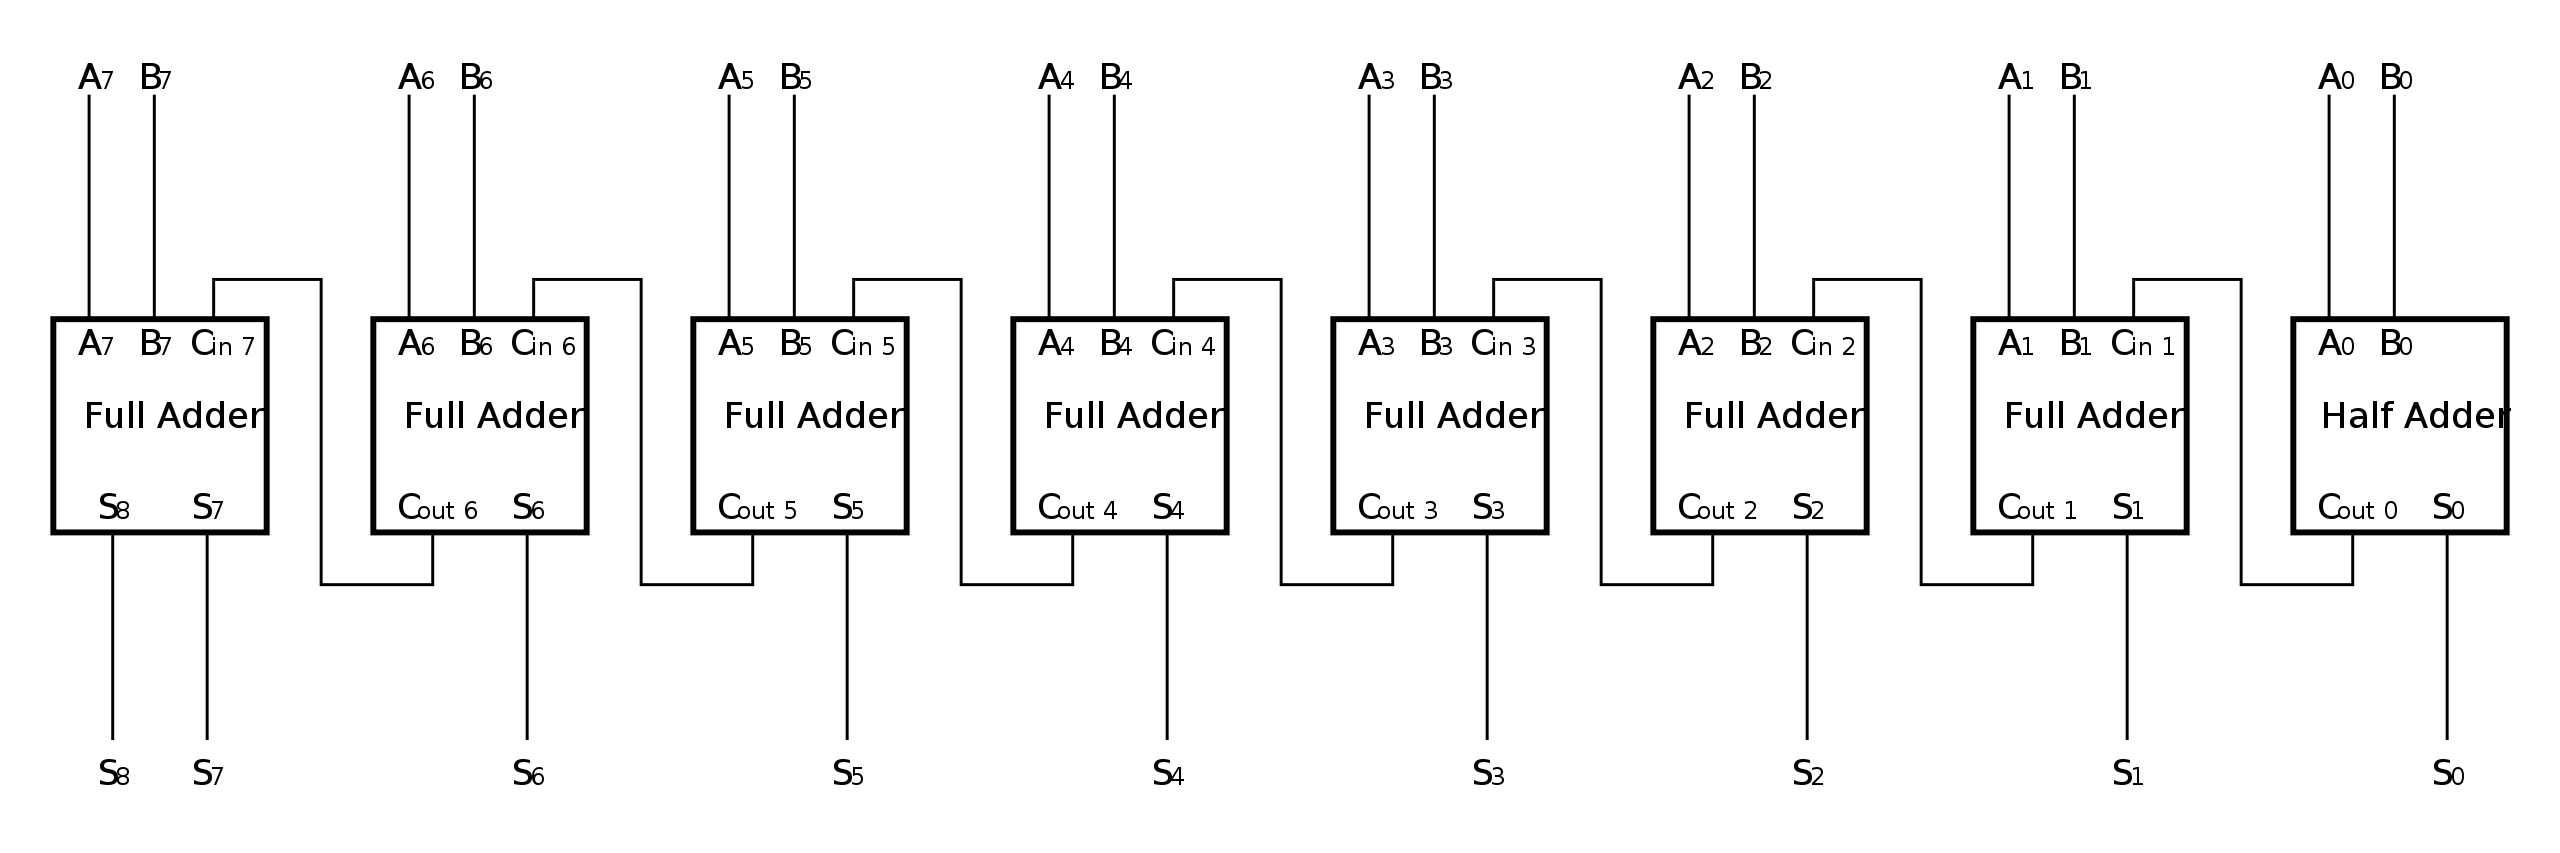
\includegraphics[width=0.95\linewidth]{../src/images/Circuit.png}
    \caption{8-bit Adder}\label{circuit}
\end{figure}
\vfill
%\subsection{Implementation}
\subsubsection{Project structure}
The project will be developed using \textit{Python 3.9.10} and we will use functions provided in the GitHub repo \url{https://github.com/ojroques/garbled-circuit}\label{ref:git}.\\
There is also a dedicated GitHub page related to this project at \url{https://github.com/lorenzozanolin/garbledCircuit}\label{zanoGit}.\\ \\
The project has the following structure:\\
\fbox{
    \begin{minipage}{40em}
    \dirtree{%
    .1 src/..
    .2 Makefile.
    .2 images \hspace{5cm} \begin{minipage}[t]{10cm}
        This directory contains the images used{.}
        \end{minipage}.
    .3 8-bit\_full\_adder.png.
    .3 Circuit.png.
    .3 Half\_adder.png.
    .3 Full-adder.png.
    .2 circuits \hspace{4.5cm} \begin{minipage}[t]{10cm}
        This directory contains the circuit used{.}
        \end{minipage}.
    .3 add.json.
    .2 code \hspace{5cm} \begin{minipage}[t]{10cm}
        This directory contains the code used{.}
        \end{minipage}.
    .3 util.py.
    .3 yao.py.
    .3 ot.py.
    .3 requirements.py.
    .3 main.py.
    .2 sets \hspace{5cm} \begin{minipage}[t]{10cm}
        This directory contains the sets saved{.}
        \end{minipage}.
    .3 alice.txt.
    .3 bob.txt.
    }
    \end{minipage}
}\\

The \inlinecode{code} folder contains all the file that we will utilize for the secure communication. \inlinecode{ot.py, util.py, yao.py} are utilities taken from \hyperref[ref:git]{Ojroques repo}.
\subsubsection{Coding}
First thing first, we need to represent the circuit; we decided to create the \inlinecode{add.json} file to code the circuit. Each wire is mapped to a number and linked with the other following the structure represented in Figure \ref{circuit}.\\
We then created \inlinecode{class Alice, class Bob} in \inlinecode{main.py} to represent their behaviour.
It was decided that both parties have command line user interaction with the user, so we developed \inlinecode{askForInput} in \inlinecode{requirements.py}. In the same file we can also find two functions \inlinecode{saveSet, readSet} used to write in two external files \inlinecode{sets/alice.txt} and \inlinecode{sets/bob.txt} the input values; this will be useful when we want to check the correctness of the computed result, using \inlinecode{verifyOperation}.\\
Since the communication is encrypted, we decided to use \textit{AES-CBC} as technique; we can see that in the file \inlinecode{yao.py}, more precisely in the two functions \inlinecode{encrypt, decrypt}. As written in the code, we opted to prepend the IV at the cyphertext to avoid reusing the same IV for all the communications.\\
We can represent the pseudocode that represents the behaviour listed before.\\

\begin{minipage}{0.46\textwidth}
    \begin{algorithm}[H]
        \centering
        \caption{Alice's behaviour}\label{alice:algo}
        \begin{algorithmic}[1]
            \State $send(circuit)$  
            \State $aliceSet \gets askForInput()$ 
            \State $saveSet(aliceSet)$ 
            \State
            \State $aliceValue \gets sum(aliceSet)$
            \State $aliceE \gets encrypt(aliceValue)$
            \State
            \State $r \gets OT.getResult(aliceE,bKeys)$
            \State
            \State $result = decimal(r)$
            \State $msg \gets verifyOperation(result)$ 
            \State $sendToBob(msg)$
            \State $printResult(result,msg)$

        \end{algorithmic}
    \end{algorithm}
    \end{minipage}
    \hfill
    \begin{minipage}{0.46\textwidth}
    \begin{algorithm}[H]
        \centering
        \caption{Bob's behaviour}\label{bob:algo}
        \begin{algorithmic}[1]
            \State $receive(circuit)$  
            \State $bobSet \gets askForInput()$ 
            \State $saveSet(bobSet)$ 
            \State
            \State $bobValue \gets sum(bobSet)$
            \State
            \State $OT.sendResult(bobValue)$
            \State
            \State $msg \gets receive()$
            \State $printResult(msg)$

        \end{algorithmic}
    \end{algorithm}
    \end{minipage}

\section{Usage}
We will briefly explain how to install the program and how it works. In my hyperref[zanoGit]{repo} there is also a graphical visualization of the executing program. 
\subsection{Installation}
To run the program you need some packages:
\begin{itemize}
    \item ZeroMQ used in \inlinecode{util.py} to implement communication;
    \item SymPy to use prime numbers;
    \item AES from encryption.
\end{itemize}
Simply run:\\
\inlinecode{\$ pip3 install pyzmq cryptography sympy}
\subsection{Communication}
\subsubsection{Example}





\bibliography{thud}
\end{document}